\documentclass{article}\usepackage[]{graphicx}\usepackage[]{color}
%% maxwidth is the original width if it is less than linewidth
%% otherwise use linewidth (to make sure the graphics do not exceed the margin)
\makeatletter
\def\maxwidth{ %
  \ifdim\Gin@nat@width>\linewidth
    \linewidth
  \else
    \Gin@nat@width
  \fi
}
\makeatother

\definecolor{fgcolor}{rgb}{0.345, 0.345, 0.345}
\newcommand{\hlnum}[1]{\textcolor[rgb]{0.686,0.059,0.569}{#1}}%
\newcommand{\hlstr}[1]{\textcolor[rgb]{0.192,0.494,0.8}{#1}}%
\newcommand{\hlcom}[1]{\textcolor[rgb]{0.678,0.584,0.686}{\textit{#1}}}%
\newcommand{\hlopt}[1]{\textcolor[rgb]{0,0,0}{#1}}%
\newcommand{\hlstd}[1]{\textcolor[rgb]{0.345,0.345,0.345}{#1}}%
\newcommand{\hlkwa}[1]{\textcolor[rgb]{0.161,0.373,0.58}{\textbf{#1}}}%
\newcommand{\hlkwb}[1]{\textcolor[rgb]{0.69,0.353,0.396}{#1}}%
\newcommand{\hlkwc}[1]{\textcolor[rgb]{0.333,0.667,0.333}{#1}}%
\newcommand{\hlkwd}[1]{\textcolor[rgb]{0.737,0.353,0.396}{\textbf{#1}}}%
\let\hlipl\hlkwb

\usepackage{framed}
\makeatletter
\newenvironment{kframe}{%
 \def\at@end@of@kframe{}%
 \ifinner\ifhmode%
  \def\at@end@of@kframe{\end{minipage}}%
  \begin{minipage}{\columnwidth}%
 \fi\fi%
 \def\FrameCommand##1{\hskip\@totalleftmargin \hskip-\fboxsep
 \colorbox{shadecolor}{##1}\hskip-\fboxsep
     % There is no \\@totalrightmargin, so:
     \hskip-\linewidth \hskip-\@totalleftmargin \hskip\columnwidth}%
 \MakeFramed {\advance\hsize-\width
   \@totalleftmargin\z@ \linewidth\hsize
   \@setminipage}}%
 {\par\unskip\endMakeFramed%
 \at@end@of@kframe}
\makeatother

\definecolor{shadecolor}{rgb}{.97, .97, .97}
\definecolor{messagecolor}{rgb}{0, 0, 0}
\definecolor{warningcolor}{rgb}{1, 0, 1}
\definecolor{errorcolor}{rgb}{1, 0, 0}
\newenvironment{knitrout}{}{} % an empty environment to be redefined in TeX

\usepackage{alltt}
\title{Stat159 Project 3: College Recommendation}
\author{Liang Hao, Bret Hart, Andrew Shibata, Gary Nguyen}
\date{\today}

\usepackage{hyperref}
\IfFileExists{upquote.sty}{\usepackage{upquote}}{}
\begin{document}

\maketitle
\section{Data}



\subsection{Description}

The data used in the construction of this app originates from the \emph{College Scorecard} database, which is developed by the U.S. Department of Education (under Obama's Administration) to provide "key indicators about the cost and value of institutions across the country to help students choose a school that is well-suited to meet their needs, priced affordably, and is consistent with their educational and career goals." The dataset can be accessed here: \href{https://collegescorecard.ed.gov/data/}(https://collegescorecard.ed.gov/data/).

\subsection{Cleaning}
For our purpose, we interpret and intercalate the data from the past five years, cleaning and merging the sets by implementing the following algorithm:\newline

1: For each dataset, we extract the columns and rows with less than 10\% \emph{PrivacySuppressed} or \emph{NaN} to obtain usable datasets with each column posessing enough information to be meaningful. We then take the unions and overlaps of the columns and rows across the years. This leaves us with around 600 columns and 6700 colleges.\newline


2: We examine the data dictionary and relevant literature, noting useful columns that may be relevant to our response variable. This arbitrarion process decreases the number of columns to under 300. We then parse the five datasets with the logically collected columns and rows.\newline

3: While we include five years of data to ease out short-term variances, we still believe more recent data has value in this circumstance, so we combine the five datasets with the following weights:

\begin{table}[ht]
\centering
\begin{tabular}{rrrrrr}
  \hline
 & Year 14-15 & Year 13-14 & Year 12-13 & Year 11-12 & Year 10-11 \\ 
  \hline
Weight & 0.40 & 0.30 & 0.10 & 0.05 & 0.05 \\ 
   \hline
\end{tabular}
\end{table}


4: Lastly, we merge the combined dataset with the \emph{Post-Graduation Salary} dataset, which contains various variables not included in the original database (despite its insane size) to form the data frame used in this project. 

\subsection{Exploratory Data Analysis}

\subsubsection{Geographical Distribution}
To gain a better sense of what we want students to input or what we should include as an important piece in the response metric, We carry out substantial exploratory data analysis. We begin by looking at colleges around the country as a whole.\newline

First, let's look at the geographical distribution of colleges in the dataset. (For the purpose of efficient  and realistic graphing, the plot unfortunately only shows colleges present in the mainland United States.

\begin{knitrout}
\definecolor{shadecolor}{rgb}{0.969, 0.969, 0.969}\color{fgcolor}

{\centering 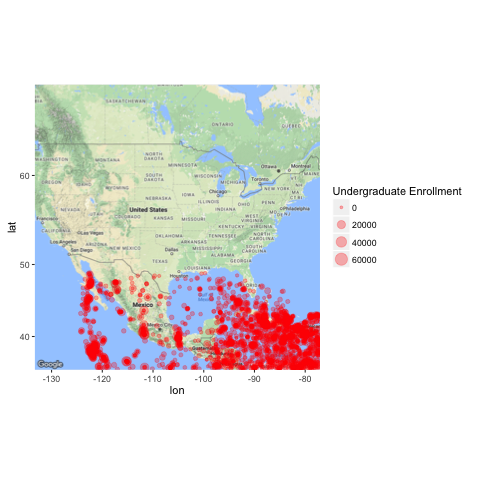
\includegraphics[width=300px]{../images/ggmap-schoolDistribution} 

}



\end{knitrout}

We see that there are a good number of schools of substantial size in most states, with the mid-western, mountain hemisphere perhaps a little low on number of educational institutions.\newline

Then, we may look at the "difficulty" of schools around the country, that is, the rejection rates, from 0\% to 100\%. 

\begin{knitrout}
\definecolor{shadecolor}{rgb}{0.969, 0.969, 0.969}\color{fgcolor}

{\centering 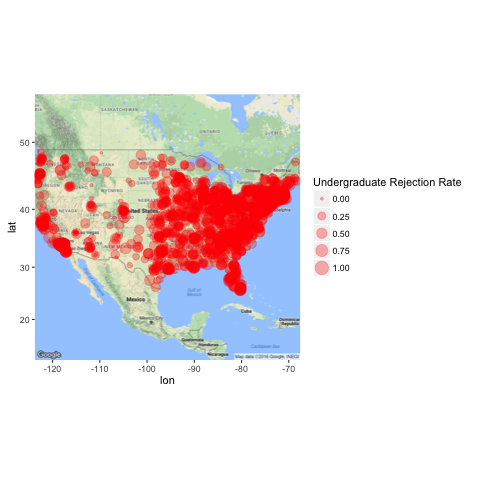
\includegraphics[width=300px]{../images/ggmap-admissionRateDistribution} 

}



\end{knitrout}

It's hard to tell as the points are smaller for lower acceptance rates, but there honestly doesn't seem to be a deficiency anywhere in schools that are, perhaps, easier to get in to, but which will undoubtedly provide a good education - this is exactly what we wanted to know. Is it even worth it to work on this recommendation platform at all? Yes, because students may have schools in their own backyards that they just need to be told about to explore and succeed. 

\subsubsection{Ethnicity}

It is no secret that those of minority racial/ethnic status in the United States may not be given the same institutional affordances in the college process, from admissions to graduation to post-graduation achievement. Even beyond negative and arbitrary admissions processes, it has been theorized that the existence of a community which is composed of students of your background, etc. can have a profound effect on success. Thus, we can examine the various ways race has been historicized in the college process, as it is and always will be of great public concern. Additionally, due to our NGO affiliation, we want to approach these institutional inequalities with a constructive open mind and a tool which suggests schools of better, or at least matching, diversity. 


\begin{table}[ht]
\centering
\begin{tabular}{rlrr}
  \hline
 & HBCU & Frequency & RelativeFrequency \\ 
  \hline
1 & No & 6613 & 0.98 \\ 
  2 & Yes & 102 & 0.02 \\ 
   \hline
\end{tabular}
\caption{Percentages of Historically Black Colleges and Universities} 
\end{table}
\begin{table}[ht]
\centering
\begin{tabular}{rlrr}
  \hline
 & PBI & Frequency & RelativeFrequency \\ 
  \hline
1 & No & 6622 & 0.99 \\ 
  2 & Yes &  93 & 0.01 \\ 
   \hline
\end{tabular}
\caption{Percentages of predominantly Black Institutions} 
\end{table}
\begin{table}[ht]
\centering
\begin{tabular}{rlrr}
  \hline
 & ANNHI & Frequency & RelativeFrequency \\ 
  \hline
1 & No & 6680 & 0.99 \\ 
  2 & Yes &  35 & 0.01 \\ 
   \hline
\end{tabular}
\caption{Percentages of predominantly Pacific Islander Institutions} 
\end{table}
\begin{table}[ht]
\centering
\begin{tabular}{rlrr}
  \hline
 & HSI & Frequency & RelativeFrequency \\ 
  \hline
1 & No & 6368 & 0.95 \\ 
  2 & Yes & 347 & 0.05 \\ 
   \hline
\end{tabular}
\caption{Percentages of predominantly Hispanic Institutions} 
\end{table}
\begin{table}[ht]
\centering
\begin{tabular}{rlrr}
  \hline
 & TRIBAL & Frequency & RelativeFrequency \\ 
  \hline
1 & No & 6684 & 1.00 \\ 
  2 & Yes &  31 & 0.00 \\ 
   \hline
\end{tabular}
\caption{Percentages of predominantly Native American Institutions} 
\end{table}
\begin{table}[ht]
\centering
\begin{tabular}{rlrr}
  \hline
 & AANAPII & Frequency & RelativeFrequency \\ 
  \hline
1 & No & 6586 & 0.98 \\ 
  2 & Yes & 129 & 0.02 \\ 
   \hline
\end{tabular}
\caption{Percentage of predominantly Asian American, Native American, Pacific Islander-serving Institutions} 
\end{table}


From these tables, we gathered that minority groups are underrepresented in the vast majority of institutions, and thus, these students may feel out of place in an environment that is mostly made up of people different than them. As a contrast to these damning tables, we offer a simple pie chart which shows racial/ethnic demographics across the schools.

\begin{knitrout}
\definecolor{shadecolor}{rgb}{0.969, 0.969, 0.969}\color{fgcolor}

{\centering 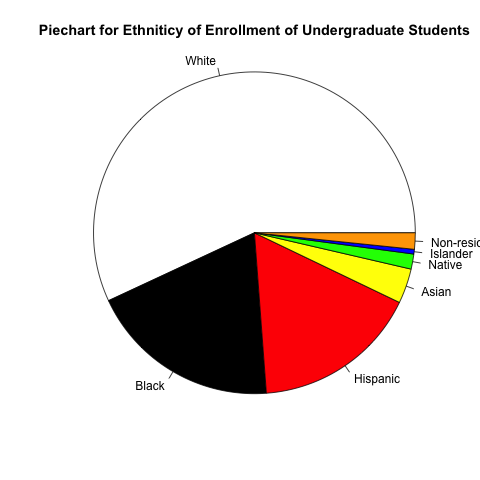
\includegraphics[width=250px]{../images/piechart-enrollmentEthnicity} 

}



\end{knitrout}

From the pie chart above, we may see that, while it is of course a problematic and contentious postulation, that white students make up the largest majority of the student body - thus, our metric of predominance in an institution may be unrealistic or not the greatest actual marker of diversity. 

\subsubsection{Net Price}
Net price is the final cost of attending an institution, which includes the amount required for tuition and fees, books and supplies, and living expenses after financial aid which would be on-default given to certain income levels. Thus, the Net Price is different for each income bracket - and our model reflects this, by pulling from different columns for net price in response to the student's input. For this project, we are obviously interested in the Average Net Price for full-time, first-time undergraduate Title IV-receiving students.\newline

Average net price $(NPT4 *$ for $PUB$ [public colleges; for public institutions, this metric is limited to those undergraduates who pay in-state tuition] and $PRIV$ [private colleges]) contains a weighted average of the net cost of attendance for all full-time, first-time undergraduate Title IV-receiving students.\newline

Here, summary statistics are provided for both Private and Public Institutions.\newline

\begin{table}[ht]
\centering
\begin{tabular}{rrrrrrrrrr}
  \hline
 & Min. & Max. & Range & Median & 25th & 75th & IQR & Mean & SD \\ 
  \hline
Public & 126.32 & 27055.80 & 26929.48 & 8604.50 & 6217.02 & 12397.31 & 6180.28 & 9444.23 & 4466.77 \\ 
  Private & 639.00 & 74245.42 & 73606.42 & 18337.28 & 13233.46 & 22543.12 & 9309.66 & 18143.31 & 7037.34 \\ 
   \hline
\end{tabular}
\caption{Summary Statistics for Net Price of Public and Private Institutions} 
\end{table}


From the table above, we (logically) see that the Net Price of Private Colleges is much higher than that of Public Colleges. As you can see, every summary statistic for Private Colleges is larger than the equivalent value for Public Colleges by a factor of 3 or 4.\newline

The following are the histograms for Net Price of both Public and Private colleges by income bracket.



{\centering 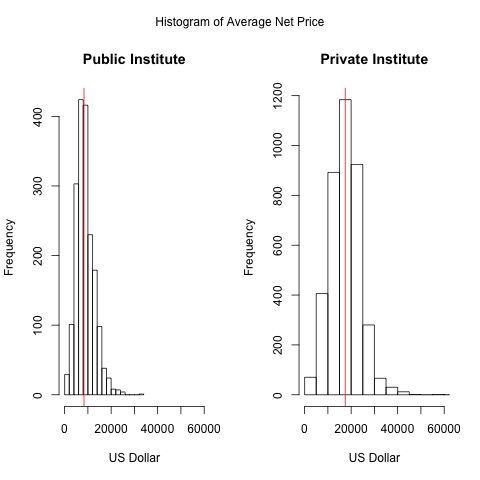
\includegraphics[width=150px]{../images/histogram-meanNetPrice} 

}




By comparing the 2 histograms, we can see that the simplified distribution of net price for public institutions is skewed-left, while net price of private colleges tends to follow a more normal-appearing distribution. \newline

The data reflects these differences by having stored many different net prices - average net price is categorized into different income quintiles for students. 

\begin{itemize}
\item USD 0 - 30,000
\item USD 30,001 - 48,000
\item USD 48,001 - 75,000
\item USD 75,001 - 110,000
\item USD 110,000+
\end{itemize}

Each quintile is further divided into 'Public' or 'Private'. 

\subsubsection{Standardized Test Scores}

Standardized Test Scores are an obvious piece of data that we could have students input into the Shiny App - weighing down schools they are substantially below the average for could definitely make a better model. This information is definitely more relevant to how likely a student may get admission rather than including as a positive metric of "quality" in the response variable. So, let's begin by looking at the general distribution of SAT and ACT scores.



{\centering 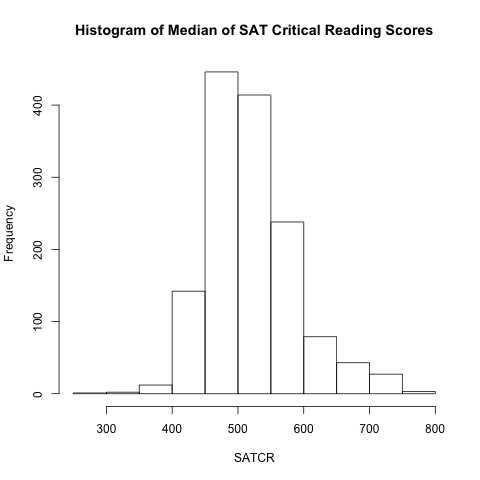
\includegraphics[width=150px]{../images/histogram-SATCRMedian} 

}


\begin{table}[ht]
\centering
\begin{tabular}{rrrrrrrrrr}
  \hline
 & Min. & Max. & Range & Median & 25th & 75th & IQR & Mean & SD \\ 
  \hline
1 & 298.00 & 757.25 & 459.25 & 511.50 & 475.50 & 556.25 & 80.75 & 520.90 & 66.81 \\ 
   \hline
\end{tabular}
\caption{Summary Statistics for SAT Critical Writing} 
\end{table}


From the histogram and the table above, we see that the median of SAT Critical Reading scores appears to have an approximately normal distribution, with the most frequent range of scores between 450 and 550. \newline

We could consider colleges with score higher than 556 to be outstanding (or, difficult to get in to) - but this would be a controversial, unfounded claim, so we mostly use the scores as metrics for the chances a student may or may not get in. Under considerable thought and some research, we decide to not weight up schools that have higher average test scores.



{\centering 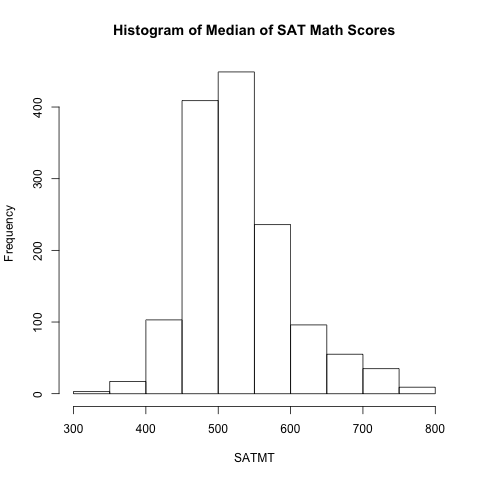
\includegraphics[width=150px]{../images/histogram-SATMTMedian} 

}


\begin{table}[ht]
\centering
\begin{tabular}{rrrrrrrrrr}
  \hline
 & Min. & Max. & Range & Median & 25th & 75th & IQR & Mean & SD \\ 
  \hline
1 & 305.00 & 783.75 & 478.75 & 516.00 & 482.31 & 563.17 & 80.86 & 528.66 & 70.38 \\ 
   \hline
\end{tabular}
\caption{Summary Statistics for SAT Math} 
\end{table}


The data for the math section of the SAT follows almost identical distribution to the Critical Reading, with the same most common range [450-550] and around a value of 553 for exceptionally difficult schools. We maintain the same decision as discussed above.\newline

Because a significant portion of colleges did not record or submit their SAT Writing scores to the original dataset, we don't analyze their distribution here.\newline

We may conduct similar analysis on reported ACT scores:



{\centering 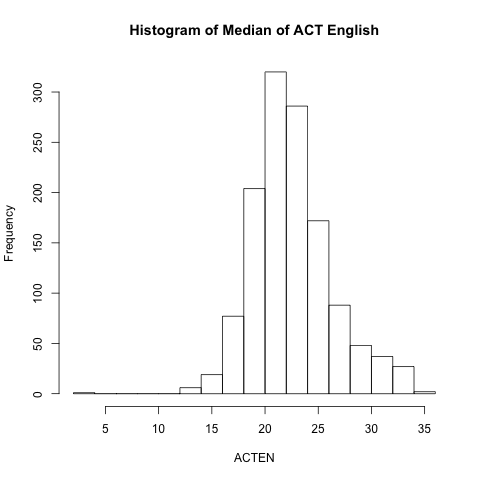
\includegraphics[width=150px]{../images/histogram-ACTENMedian} 

}


\begin{table}[ht]
\centering
\begin{tabular}{rrrrrrrrrr}
  \hline
 & Min. & Max. & Range & Median & 25th & 75th & IQR & Mean & SD \\ 
  \hline
1 & 2.00 & 34.40 & 32.40 & 22.17 & 20.16 & 24.60 & 4.44 & 22.69 & 3.78 \\ 
   \hline
\end{tabular}
\caption{Summary Statistics for ACT English} 
\end{table}


From the histogram and the table above, we can see that the median of ACT English scores basically follows a normal distribution, with most of the scores clustering between 20 and 24. We may consider colleges with such score higher than 24.6 to be exceptionally difficult to get in to.



{\centering 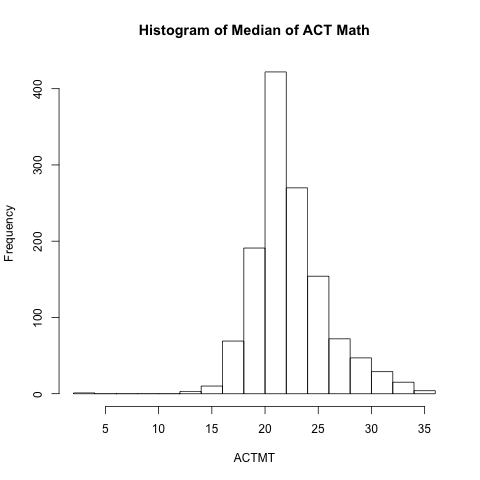
\includegraphics[width=150px]{../images/histogram-ACTMTMedian} 

}


\begin{table}[ht]
\centering
\begin{tabular}{rrrrrrrrrr}
  \hline
 & Min. & Max. & Range & Median & 25th & 75th & IQR & Mean & SD \\ 
  \hline
1 & 2.00 & 35.40 & 33.40 & 21.95 & 20.40 & 24.00 & 3.60 & 22.47 & 3.41 \\ 
   \hline
\end{tabular}
\caption{Summary Statistics for ACT Math} 
\end{table}



Lastly, we examine the ACT math distribution. We can see that the median of ACT Math scores basically follows a normal distribution, with most of the scores clustering between 20 and 24, and an average score higher than 24 appears to represent a school exceptionally difficult to attend.\newline

As discussed in the critical reading section, upon substantial thought, we decide that these scores may not be perfect, empirical markers of institutional quality, so we hesitate to include them in our baseline composite response metric. We do include scores, though, as an input that a student can manipulate. In our final app, if their score is lower than the average for that institution, the score for the school will be weighted down but still shown. This is not functionally equivalent to just including the average score in our response variable and weighting up schools that have higher ones, so we are much more satisfied with this method of including scores, as they definitely matter for college admissions. Thus, we are not suggesting that test scores are unimportant to the college process, but that they may not be great markers of objective quality. We include them only out of fairness to students, as recommending schools that they may not be qualified to apply to would be against our mission statement. We don't rule these schools out completely, instead, merely hesitating to immediately reccomend them, as they may have other statistics that make them strong potential schools, but out of reach of most applicants.\newline

Though this is representative of only a subsection of our research and exploratory analysis, we include this section as demonstration of our arduous process in determing what would be good to include in our model, both as part of our responsive "quality score" or as inputs for students, so they can be shown schools with student bodies more similar to who they are or schools that they could realistically get in to. Thus, this exploratory analysis was invaluable in getting a sense of some information about schools across the nation to inform our modeling decisions. \newline

To explain some actual decisions we made from this exploratory analysis, we decide to heavily include geographic location in determining output for students, as in-state tuition for public schools is more readily available in the dataset and out-of-state net price may not be as consistently available. Thus, if we wish to realistically model the net prices of public schools, we can only do so if the student is a resident of that state. This may be a minor shortcoming of our model, but it is a data limitation, not a creative one! Ethnicity of the student body in relation to a student's own is included in the model, as research indicates that attending a school with students of your racial/ethnic background can greatly improve comfort, success, retention, etc. Net price is obviously included in our response for obvious reasons - we can't, in good faith, recommend at-risk students to apply to schools with significantly higher net prices, as net price actually represents the *final cost* of attendance after financial aid for each income bracket. Thus, it can included wholesomely and in good faith. Our last main piece of information analyzed, SAT/ACT scores, we decided were not worth including in our baseline model as quality indicators due to their imperfection. We begrudgingly but out of necessity include them as inputs for students that alter schools shown out of a desire to maintain an honest, truthful relationship with the students, showing them schools that are worth the application. Again, our mission is to create an interactive list of schools which are high-quality at a low-cost for students who need the help.  

\end{document}
